\section{Gestion de projet}

\paragraph{}
Cette partie consiste à exposer la manière dont nous nous sommes organisés pour la réalisation de ce projet. Ce sujet de PIE s'inscrit globalement dans une stratégie commune de recherche entre l'ISAE-SUPAERO et l'ONERA. L'objectif est l'amélioration du code de calcul JAGUAR basé sur les différences spectrales ayant pour objectif d'effectuer des simulations numériques LES pour des applications CFD.

\paragraph{}
Les méthodes spectrales discontinues consistent à représenter la solution par cellule de calcul sur une base polynômiale et à prendre en compte la discontinuité de la solution entre cellules par résolution d'un problème de Riemann. Assez récentes en CFD, leurs applications pour la LES est un sujet de recherche actuel. Aujourd'hui, les études se focalisent essentiellement sur la précision des schémas spatiaux pour la convection et la diffusion. Ici, on souhaite focaliser notre attention sur les schémas numériques d'intégration temporelle des équations dans un code prototype 1D. Après une analyse bibliographique sur les méthodes temporelles, nous proposons l'implémentation de plusieurs familles de schémas dans une maquette 1D puis de comparer les performances.

\subsection{Description du projet}

    \subsubsection{Objectifs du projet et résultats attendus}
        \paragraph{}
        Une première liste des objectifs attendus par le client est énumérée ci-après :
        \begin{itemize}
            \item une analyse bibliographique des différentes classes de méthodes
            \item une analyse approfondie des schémas numériques (précision, coût algorithmique, CFL max) 
            \item une maquette dans laquelle les schémas sont implémentés et plusieurs cas tests de validation 
            \item un rapport sur la comparaison croisée des schémas numériques
            \item une liste de recommandations du groupe sur le(s) meilleur(s) schéma(s)
        \end{itemize}

        \paragraph{}
        Afin de répondre au cahier des charges client nous devons implémenter les méthodes numériques en langage Python. Sur les conseils de notre client nous avons utilisé la plateforme de travail GitHub qui est très adaptée, pour travailler sur des fichiers de code informatique notamment. Ceci nous permet aussi d'avoir plusieurs sauvegardes de notre travail et cela prévient donc d'une éventuelle perte du code informatique.

        \paragraph{}
        La documentation détaillée du code est une requête du client c'est pourquoi nous avons utilisé le logiciel libre Sphinx pour créer la documentation du code. Ce programme, simple d'utilisation, permet de compiler une documentation au format \emph{html}, constituée de pages détaillées, comportant des fonctionnalités de navigation par lien hypertexte.

    \subsubsection{Les parties prenantes du projet}
        \paragraph{}
        Il est important de bien connaître toutes les parties prenantes du projet afin que la communication entre ces différentes parties soit fluide et efficace.
        \begin{itemize}
            \item Louis Reboul, Pierre Seize, Sara Barrasa-Ramos, Jean-Baptiste Fourtout et Théo Maes : groupe d'étudiants de L'ISAE qui représente l'équipe de développeurs
            \item Guillaume Puigt : Client et encadrant technique de l'ONERA
            \item Xavier Vasseur : Client, encadrant technique et référent école
            \item Rémi Lebouteiller : Tuteur en gestion de projet
        \end{itemize}

        \paragraph{}
        Dans le but de garantir une bonne communication avec les différentes parties nous avons mis en place plusieurs interfaces de communication. Néanmoins nous les détaillerons un peu plus loin dans ce rapport.

    \subsubsection{Les contraintes identifiées}
        \paragraph{}
        Les contraintes connues portent sur l'environnement de développement du code informatique, elles sont imposées par le client :
        \begin{itemize}
            \item utilisation du langage de programmation Python, version 2.7
            \item Utilisation de la plateforme GitHub pour la gestion du versionnage des fichiers
        \end{itemize}

    \subsubsection{Hypothèses de travail}
        \paragraph{}
        Les hypothèses du projet portent sur les ressources disponibles et la capacité de travail des membres de l'équipe de développement.
        \begin{itemize}
            \item L'équipe de développement peut fournir 4h à 8h de travail par semaine et par personne.
            \item La bibliographie est fournie par Guillaume Puigt et par Xavier Vasseur.
            \item Les algorithmes d'intégration spatiales sont fournis par Guillaume Puigt.
        \end{itemize}

        \paragraph{}
        Ayant identifié tous les objectifs et les contraintes associées, il nous faut établir une stratégie afin de se répartir la charge de travail de façon équivalente au sein de l'équipe.


\subsection{Organisation}

    \subsubsection{Outils de gestion de projet}
        \paragraph{}
        Les outils qui nous ont été très utiles pour mettre des limites à notre projet et de répartir les différentes tâches au sein de l'équipe sont principalement les diagrammes PBS et WBS.

        \paragraph{}
        Le diagramme PBS (Product Breakdown Structure) nous permet de savoir dans quelle ordre nous allons effectuer les différentes opérations pour aboutir à l'objectif du projet (figure \ref{PBS}).
        \begin{figure}
            \centering
            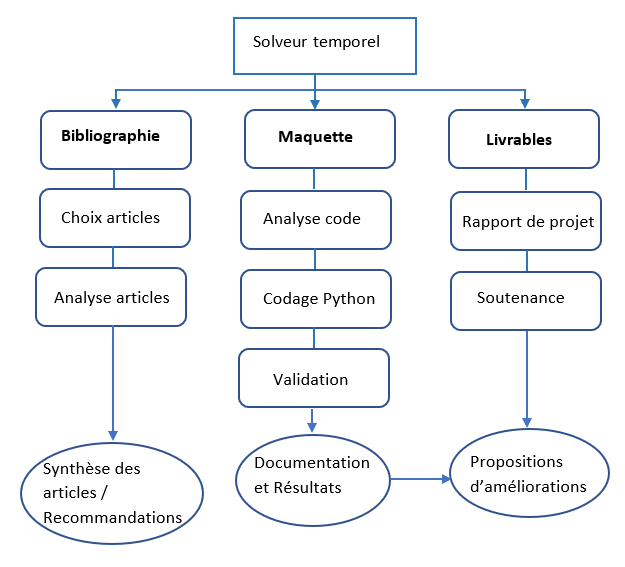
\includegraphics[width=0.6\textwidth]{images/pbs.png}
            \caption{Diagramme PBS}
            \label{PBS}
        \end{figure}

        \paragraph{}
        D'un autre côté, le diagramme WBS (Working Breakdown Structure) nous indique plutôt comment nous allons effectuer ces opérations. Cela permet de définir différentes tâches et nous répartir le travail de manière équitable pour lisser la charge de travail sur chacun des membres de l'équipe (figure \ref{WBS}).
        \begin{figure}
            \centering
            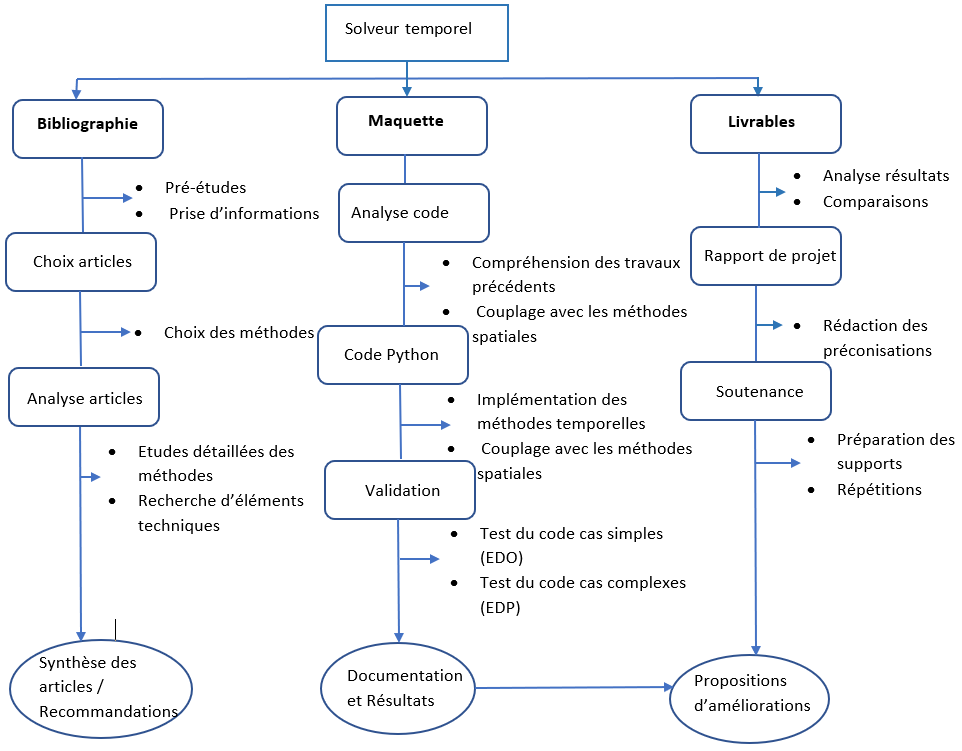
\includegraphics[width=0.8\textwidth]{images/wbs.png}
            \caption{Diagramme WBS}
            \label{WBS}
        \end{figure}

        \paragraph{}
        L'utilisation de ces outils nous a permis de délimiter le périmètre de travail afin de rester focalisé sur l'objectif du client et de ne pas divaguer. Ici le diagramme WBS (figure \ref{WBS}) n'est pas détaillé à son maximum par soucis de lisibilité. Cet outil donne une bonne idée d'ensemble de toutes les tâches qui sont à réaliser dans un ordre précis pour aboutir au résultat final du projet. 

    \subsubsection{Organisation de l'équipe}
        \paragraph{}
        La répartition du travail s'est faite assez naturellement en deux équipes grâce aux diagrammes PBS et WBS vu précédemment. Nous connaissions très bien les limites de notre projet et les étapes à effectuer pour parvenir aux objectifs du client. Chacun a pu trouver sa place au sein de la configuration suivante (figure \ref{fig:OBS}):
        \begin{itemize}
            \item Théo Maes est le chef de projet.
            \item L'équipe développement, coordonnée par Sara Barrasa-Ramos, sera responsable de l'implémentation des méthodes numériques. Elle sera composée de :
            \begin{itemize}
                \item Louis Reboul,
                \item Sara Barrasa-Ramos,
                \item Théo Maes.
            \end{itemize}
            \item L'équipe couplage, coordonnée par Pierre Seize, sera responsable de rendre compatible les schémas numériques d'intégration temporelle avec les schémas numériques d'intégration spatiale existants. Elle sera composée de :
            \begin{itemize}
                \item Pierre Seize,
                \item Jean-Baptiste Fourtout.
            \end{itemize}
        \end{itemize}
        \begin{figure}
            \centering
            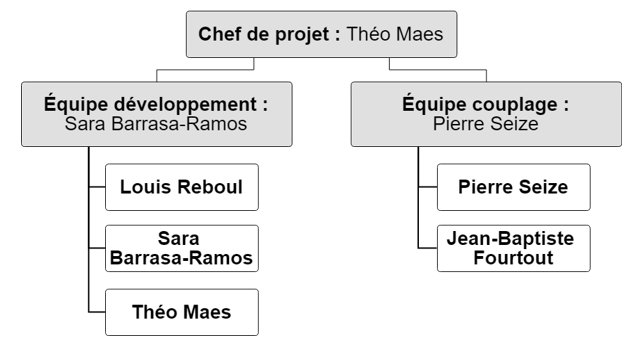
\includegraphics[scale=0.7]{images/obs.png}
            \caption{Organisation de l'équipe} 
            \label{fig:OBS}
        \end{figure}

        \paragraph{}
        Cette répartition ayant été faite en consensus avec l'ensemble de l'équipe, en prenant en compte les préférences de chacun et le niveau de connaissance dans ce domaine d'application des sciences. Nous nous sommes efforcés de conserver le plus possible cette répartition du travail. Néanmoins nous avons été contraints d'effectuer certains changements temporaires de ressources humaines au cours du projet pour pallier des problématiques qui seront expliquées plus en détail par la suite.

    \subsubsection{Organisation du travail}
        \paragraph{}
        Il nous semble important d'aborder la matrice RACI qui est née de l'association des diagrammes OBS et WBS. En effet, cette matrice permet de repérer le rôle de chacun des membres de l'équipe pour une tâche donnée comme il est indiqué figure \ref{fig:RACI}.

        \paragraph{}
        La lettre R signifie "Réalisation", dans le sens où les personnes assujetties à cette lettre pour une tâche doivent fournir un travail. C'est différent si la personne est associée à la lettre C, signifiant "Consultation", car cela signifie simplement qu'elle peut posséder des connaissances, un point de vue intéressant sur la réalisation de la tâche. Cette consultation est effectuée en amont de la réalisation. L'indice I pour "Information" concerne les conseils promulgués par des gens qui ont la connaissance pour améliorer la réalisation de la tâche. Et enfin la lettre A signifie "Approbation" et concerne les personnes qui vont prendre les décisions. Dans le cadre de notre projet, cela se restreint au chef d'équipe en charge de la tache en question.
        \begin{figure}
            \centering
            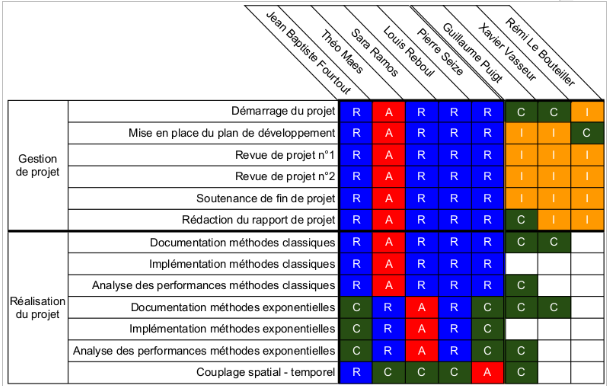
\includegraphics[width=\textwidth]{images/raci.png}
            \caption{Matrice RACI} 
            \label{fig:RACI}
        \end{figure}

        \paragraph{}
        Il est naturel que le chef de projet ne sert pas qu'à l'approbation des tâches réalisées par ses camarades, il participe au même titre que tout le monde.

        \paragraph{}
        Cette matrice est intéressante car elle permet à chacun des collaborateurs de voir avec qui il travaille sur une même tâche et de pouvoir échanger avec eux. On identifie d'autant plus rapidement les personnes "expertes" qui sauront nous orienter dans le cas d'un blocage lors de la réalisation d'une tâche.


\subsection{Processus du développement}

    \subsubsection{Logique de développement}
        \paragraph{}
        Notre logique de développement du projet s'articule principalement sur les différents groupes de tâches qui ont été répertoriés dès la mise en place du projet à l'aide des diagrammes PBS et WBS.

        \paragraph{}
        En toute logique nous avons commencé par prendre connaissance de la bibliographie qui est directement fournie par notre client. Puis il a fallu prendre en main la programmation avec le langage Python car tous les développeurs n'avaient pas la même connaissance de ce langage informatique.

        \paragraph{}
        Une analyse approfondie des articles scientifiques et des recherches personnelles du groupe ont permis à l'équipe développement de faire un choix sur les méthodes temporelles qui seront étudiées plus en profondeur. C'est sur des conseils et en accord avec notre client que nous avons fait ces choix. En parallèle l'équipe se chargeant du couplage spatial-temporel devait comprendre en profondeur le fonctionnement du code informatique fournit pour établir une stratégie pour pouvoir y adapter le travail de l'équipe développement.

        \paragraph{}
        Ensuite, nous avons implémenté les nouvelles méthodes de résolution temporelle dites "Exponentielles", pendant que l'équipe couplage testait le couplage spatial-temporel avec les méthodes usuelles que l'équipe développement a mis très rapidement en oeuvre au début du projet.

        \paragraph{}
        Une fois que l'équipe développement réussi à implémenter une méthode exponentielle, l'équipe couplage peut lancer une phase de test pour vérifier le bon fonctionnement du couplage des méthodes sur des cas simples puis plus complexes.

    \subsubsection{Définition des jalons}
        \paragraph{}
        Définition des jalons et la nature des jalons :
        \begin{itemize}
            \item 21/11/2018 : Première revue de projet, présentation orale de l'avancée des travaux.
            \item 30/01/2018 : Deuxième revue de projet, présentation orale de l'avancée des travaux accompagnée d'un début de rapport du projet.
            \item Mi-mars : Soutenance de projet, présentation orale de l'ensemble du projet et des problèmes rencontrés.
            \item Fin mars : Rendu des livrables (rapport de projet, code source).
        \end{itemize}
        \paragraph{}
        Les jalons étant fixés dès le début du projet, ils ont permis de donner un "tempo" au travail a effectuer. En complément, le diagramme WBS et les coûts associés à chaque tâche on permis de rapidement établir un premier diagramme de Gantt (figure \ref{fig:Gantt_initial}).
        \begin{figure}
            \centering
            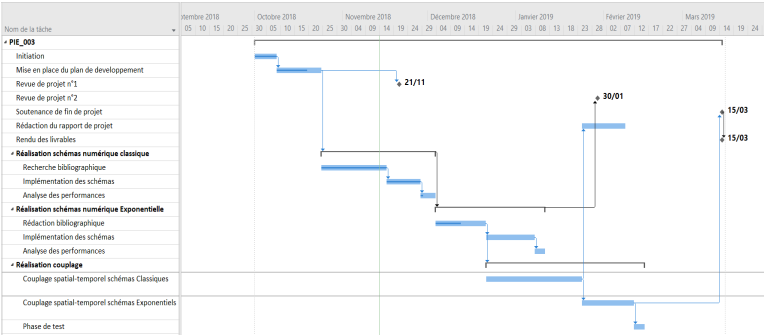
\includegraphics[width=\textwidth]{images/gantt.png}
            \caption{Diagramme de Gantt initial} 
            \label{fig:Gantt_initial}
        \end{figure}

    \subsubsection{Planning de projet}
        \paragraph{}
        Après plusieurs entretiens avec le client, nous avons convenu de plusieurs changements qui ont provoqués des différences majeures dans l'emploi du temps du projet. 

        \paragraph{}
        Nous nous occupons de la partie intégration temporelle, néanmoins cette partie doit être couplée avec les méthodes d'intégration spatiales. Ces méthodes ont été réalisées au préalable par d'autres groupes d'étudiants de Supaero dans les années antérieures. Pour l'équipe couplage, il s'est avéré difficile de reprendre le code informatique tel qu'il nous était fourni pour le coupler avec notre travail sur l'intégration temporelle. Après discussion avec nos clients, nous avons donc réussi à les convaincre de changer la structure du code afin qu'il soit plus flexible et utilisable qu'avant.

        \paragraph{}
        Cette tâche supplémentaire était un risque très important pour notre projet. Car le code informatique étant fonctionnel, nous risquions le dégrader et le rendre inutilisable. Dans un second temps cette tâche n'était pas prévue dans le diagramme de Gantt initial. Il y avait donc un risque de passer trop de temps sur cette opération et compromettre l'ensemble du projet.
        \begin{figure}
            \centering
            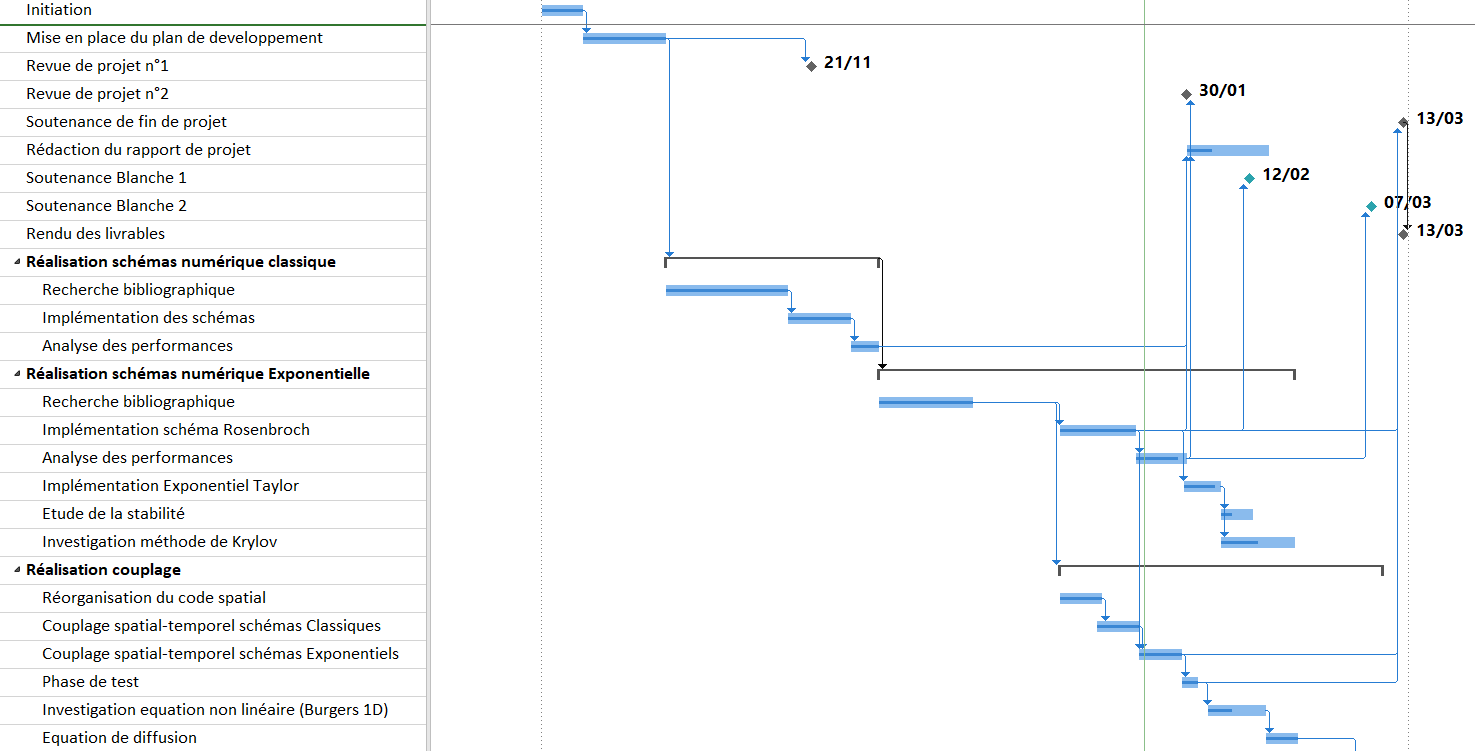
\includegraphics[width=\textwidth]{images/gantt_2.png}
            \caption{Diagramme de Gantt modifié} 
            \label{fig:Gantt modifié}
        \end{figure}

        \paragraph{}
        Finalement, comme nous pouvons le voir sur la figure \ref{fig:Gantt modifié} ce risque s'est transformé en opportunité, car la tâche a été effectuée rapidement et avec succès ce qui a permit à l'équipe couplage de gagner un temps considérable sur la suite du projet.

        \paragraph{}
        En parallèle l'équipe développement a eu des difficultés sur l'implémentation des schémas temporels. Le travail de l'équipe couplage étant conditionné par la réussite de l'équipe développement nous avons fait le choix de déplacer une ressource humaine dans l'équipe implémentation. Nous avons donc globalement pris de l'avance sur les objectifs initiaux fixés du projet. 

        \paragraph{}
        Le diagramme de Gantt est l'outil principal que nous avons utilisé tout au long du projet. Il permet de situer temporellement parlant le travail effectué par rapport aux prévisions, ce qui est très utile quand les demandes du client évoluent au cours du projet.

        \paragraph{}
        Le client a par exemple exigé des soutenances de projet "blanches" mi-février et début mars. Ceci nous a donc imposé de préparer des présentations orales supplémentaires et d'arranger la répartition du travail de façon à avoir de nouveaux  résultats à montrer au client lors de la soutenance. Ces aléas d'emploi du temps ont été très bien gérés par l'équipe grâce au diagramme de Gantt. Ces modifications apparaissent en comparant les figures \ref{fig:Gantt_initial} et \ref{fig:Gantt modifié}.


\subsection{Coût réel du projet}

    \paragraph{}
    Comme nous avons pu le voir, nous avons gagné du temps sur certaines tâches ce qui nous a permis d'aller plus loin que ce que le client demandait initialement. Néanmoins ce surplus de tâches nous a fait dépasser le nombre d'heures alloué à ce projet d'environ 20\%. Ce qui fait un total de 480h pour ce projet. En considérant la rémunération minimale d'un stagiaire qui est de 3,72 euros par heure net, le montant du projet s'élèverait à 1785,6\euro auquel s'ajouterait les charges patronales. Considérons maintenant un salaire de jeune ingénieur à la sortie de l'école ISAE-SUPAERO en se basant sur un revenu annuel de 40 000\euro brut par an. En considérant des charges patronales de l'ordre de 30\%, le montant du projet s'élèverait cette fois-ci à 9984\euro. Il faut souligner le fait que nous avons été plus loin que les objectifs initiaux et que par conséquent le prix du projet s'en fait ressentir dans la globalité.


\subsection{Les livrables du projet}

    \subsubsection{Liste des produits livrables au client}
        \paragraph{}
        Les livrables du projet sont :
        \begin{itemize}
            \item une revue bibliographique avec pour objectif de répondre aux questions : \textit{quelles méthodes est-il conseillé d'utiliser, pourquoi et pour quelles applications ?}
            \item un rapport de projet (le présent document)
            \item un rendu des supports utilisés pour la soutenance finale
            \item le code informatique avec pour critère d'acceptation d'être fait en langage Python et publié sur la plateforme GitHub
        \end{itemize}

    \subsubsection{Liste des livrables demandés par le corps enseignant}
        \paragraph{}
        Dans le cadre du module de gestion de projet de l'ISAE Supaero, nous devons rendre un plan de développement de notre projet. D'autre part nous sommes évalués sur un rapport de projet et une soutenance qui aura lieu mi-mars. Ce sont donc des livrables requis.

        \paragraph{}
        Un dernier livrable requis est une fiche synthèse, format A4, résumant brièvement les enjeux du projet et les résultats obtenus. 


\subsection{Risques et opportunités}

    \paragraph{}
    Les risques liés au projet sont répertoriés dans le tableau présenté en figure \ref{Tab risque}. On peut voir que ce tableau est réalisé en définissant pour chaque risque potentiel une occurrence et une gravité à travers un coefficient. Le produit de ces deux coefficients nous indiquera tout naturellement si l'impact du risque considéré sur le projet est fort ou non. L'utilisation d'un code couleur permet ensuite de repérer visuellement les risques majeurs d'un simple coup d'oeil.

    \paragraph{}
    Une fois ces risques identifiés, il est à notre charge de faire en sorte qu'ils ne se produisent pas. C'est donc ce que nous nous sommes efforcés de faire tout au long du projet. Bien sûr ayant une faible expérience en gestion de projet, il est difficile d'identifier en amont tous les risques qu'un projet peu présenter.

    \paragraph{}
    Il y a d'ailleurs un risque que nous n'avions pas considéré : l'incompatibilité ou la difficulté du couplage de notre travail avec la méthode spatiale. En effet, la méthode spatiale étant fournie par le client, nous avons récupéré un code informatique fonctionnel. Néanmoins ce code était réalisé de manière peu flexible et était de mauvaise qualité (d'un point de vue informatique, et pas algorithmique) ce qui ne permettait pas de coupler les deux travaux de façon simple et agile.

    \paragraph{}
    C'est alors qu'un choix s'offrait à nous : soit prendre le temps de réécrire la partie du code fournie par le client et avoir la garantie d'avoir un résultat, soit avoir des difficultés pour tester les fruits de notre travail de recherche au risque que cela nous prenne beaucoup de temps. Nous avons préféré, avec l'accord du client, reprendre la structure du code fournit afin de pouvoir effectuer un couplage de notre travail de manière propre et efficace.

    \paragraph{}
    Ce qui s'apparentait à un risque s'est transformé en opportunité car finalement, par rapport au diagramme de Gantt initial, nous avions gagné du temps. Cela nous as ensuite permis de faire plus de choses et de réellement pousser notre travail.
    \begin{figure}
        \centering
        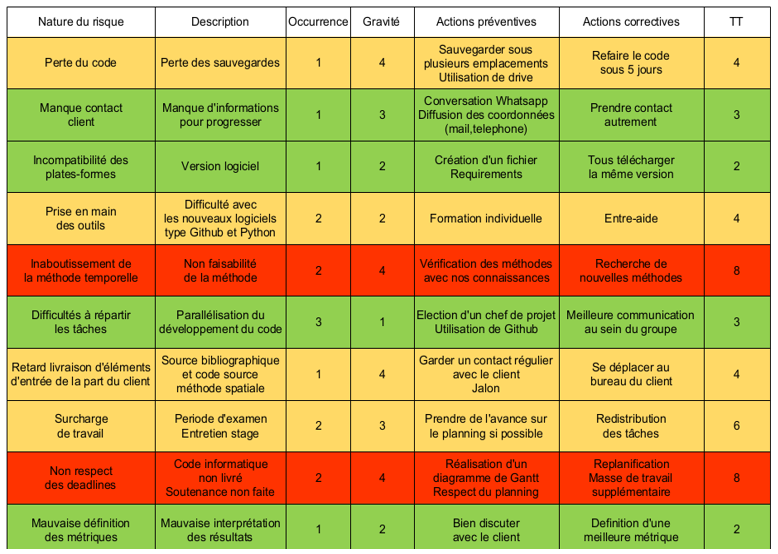
\includegraphics[width=\textwidth]{images/matrice_risque.png}
        \caption{Tableau des risques}
        \label{Tab risque}
    \end{figure}


\subsection{Suivi et Contrôle}

    \subsubsection{Tableau de bord de suivi}
        \paragraph{}
        Nous avons l'opportunité d'utiliser le logiciel MS-Project pour réaliser un suivi du projet. Nous avons réalisé un diagramme de Gantt de référence que nous avons mis à jour au fur et à mesure que le projet évoluait. Cela nous a été très utile car comme nous l'avons vu précédemment nous avons pu réagir vite à des problèmes rencontrés lors du projet.

        \paragraph{}
        Avec l'élaboration du WBS nous avions pu mettre un coût sur chaque tâche à réaliser, et le diagramme de Gantt à mis en évidence qu'en fin de projet, des personnes seraient en surcharge de travail. Nous nous sommes donc efforcés dès le début du projet à ré-agencer les tâches, mais les aléas du projet nous ont aussi aidé à résoudre ce problème.  

        \paragraph{}
        L'utilisation de la plate-forme GitHub, gérant le versionnage des fichiers, possède certaines fonctions aidant aussi à la gestion du projet. On peut rapidement voir quelle personne travaille sur quelle partie du code. Pour le partage de documents, nous avons créé un groupe sur un site de stockage et de partage de documents.

        \paragraph{}
        Ce sont autant de plate-formes qui permettent de garder l'ensemble de l'équipe en contact. Cela a aussi tendance à créer une émulsion et une dynamique de groupe. Néanmoins il faut veiller à ne pas avoir trop d'outils pour ne pas se perdre. Mais dans notre cas chacune des interfaces avait une fonction différente et bien définie

    \subsubsection{Communication}

        \paragraph{}
        De façon à être dynamiques au sein du groupe nous avons mis en place une conversation WhatsApp. L'interface utilisée pour cette application étant le smartphone, cela permet rapidement d'échanger des informations, ou de se donner rendez-vous pour travailler. Notre client est d'ailleurs membre de cette conversation, ce qui lui permet de rester en permanence au courant de l'avancée de notre travail.

        \paragraph{}
        Néanmoins, d'un point de vue plus formel, il nous paraissait très important d'utiliser les mails. C'était de plus le seul moyen de communication avec certaines parties prenantes du projet.

        \paragraph{}
        D'autre part, en moyenne, nous avions décidé de faire des réunions bimensuelles dès le début du projet. Sur l'ensemble du projet il s'agit d'une contrainte que nous nous sommes imposés mais qui fût respectée et nous a permis de rester à l'écoute de notre client concernant ses exigences, qui ont évoluées au cours du temps.

